% command to run this on the terminal is lualatex -shell-escape Pictogram_Sleep_Regulation.tex
% requires pgfplots

\pdfpxdimen=1in
\divide\pdfpxdimen by 600

\documentclass[10pt]{standalone}
\usepackage{tikz}


%has to be compiled with ``lualatex -shell-escape Pictogram_Sleep_Regulation.tex''
\usetikzlibrary{external, positioning, backgrounds, arrows.meta, decorations.pathmorphing, calc}

% set up externalization
% WARNING the name of the Image CANNOT be the same as the tex file
\tikzsetnextfilename{Pictogram_SR}
\tikzset{external/system call={lualatex \tikzexternalcheckshellescape -halt-on-error
-interaction=batchmode -jobname "\image" "\texsource";
convert -density 600 -compress LZW "\image".pdf -flatten -alpha off -colorspace RGB -depth 8 "\image".tif;
convert -density 600 "\image".tif  "\image".jpg;}}
\tikzexternalize

\begin{document}
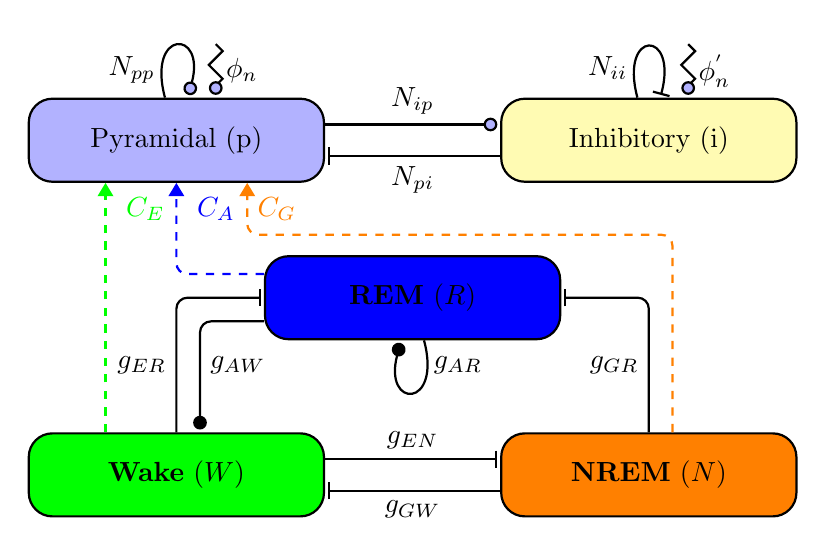
\begin{tikzpicture}[  
  s/.style  = {shorten >=1pt},
  every loop/.style={thick,shorten >=1pt},
  every path/.style={thick},
  pop/.style	 = {rectangle, draw, text width=10em, text centered, minimum height=3em, rounded corners=3mm},
  noise/.style = {decorate, decoration={zigzag},-{Circle[fill=blue!30]}, s},
  Ex/.style = {rounded corners, s, -{Circle[fill=blue!30]}},
  In/.style = {rounded corners, s, -|},
  ExSR/.style = {rounded corners, s, -{Circle}}, 
  ]
  % Cortex populations
  \node (ex)   at (0,0)		[pop, fill=blue!30]	{Pyramidal (p)};
  \node (in)   at (6,0)		[pop, fill=yellow!30]	{Inhibitory (i)};
  % Sleep regulation populations
  \node (WAKE) at (0,-4.25)	[pop, fill=green] 	{\textbf{Wake} ($W$)};
  \node (NREM) at (6,-4.25)	[pop, fill=orange]	{\textbf{NREM} ($N$)};
  \node (REM)  at (3,-2)	[pop, fill=blue]	{\textbf{REM} ($R$)};

  % Connections within cortex
  \draw
  (		   ex)	    edge [Ex, loop above] node[below left, xshift = -0.4em]	{$N_{pp}$}	(		ex)
  ([yshift= 0.2cm] ex.east) edge [Ex]		  node[above] 				{$N_{ip}$}	([yshift= 0.2cm]in.west)
  ([yshift=-0.2cm] in.west) edge [In] 	    	  node[below] 				{$N_{pi}$}	([yshift=-0.2cm]ex.east)
  (		   in)	    edge [In, loop above] node[below left, xshift = -0.4em]	{$N_{ii}$}	(		in)
  (0.5,1.22)  		    edge [noise] 	  node[right] 				{$\phi_n$}	([xshift= 0.5cm]ex.north)
  (6.5,1.22)  		    edge [noise] 	  node[right] 				{$\phi^{'}_n$}	([xshift= 0.5cm]in.north);
  
  % Connections within sleep regulation
  \draw[ExSR]
  ([yshift=-0.3cm] REM.west)	-- (0.3,-2.3) 
				-- node (N3){}	    					([xshift= 0.3cm] WAKE.north)
  (	 	   REM)	       edge[s,loop below,-{Circle}]node	(N2){} 		    	(		 REM);
  \draw[In]
  (		   WAKE.north)	-- node[left]	(N0) {$g_{ER}$}				(0.0,-2.)
				--							(		 REM.west);
  \draw[In]
  (		   NREM.north)	-- node		(N1) {}					(6,-2)
				--							(		 REM.east);
  \draw[In]
  ([yshift= 0.2cm] WAKE.east)   -- node[above]	{$g_{EN}$}				([yshift= 0.2cm] NREM.west);
  \draw[In]
  ([yshift=-0.2cm] NREM.west)	-- node[below]	{$g_{GW}$}				([yshift=-0.2cm] WAKE.east);

  % Place labels based on relative coordinates
  \draw let \p1 = (N0), \p2 = (N1), \p3 = (N2), \p4 = (N3)
	in node[right, xshift = 0.4em]	at (\x3,\y1) {$g_{AR}$}
	   node[right]  		at (\x4,\y1) {$g_{AW}$}
	   node[left]  	  		at (\x2,\y1) {$g_{GR}$};

  % The interaction between SRN and cortex  
  \draw[orange, dashed, rounded corners, -{Triangle}]
  ([xshift= 0.3cm] NREM.north)  -- (6.3, -1.2) 
			        -- (0.9, -1.2)
				-- node[right] (C1) {$C_{G}$} ([xshift= 0.9cm] ex.south);	  
  \draw[blue, dashed, rounded corners, -{Triangle}]
  ([yshift= 0.3cm] REM.west)   -- ( 0.0,-1.7)  
			       --    node[right] (C2) {} (ex.south);
  \draw[green, dashed, rounded corners, -{Triangle}]
  ([xshift=-0.9cm] WAKE.north) --   node[right] (C3) {}  ([xshift=-0.9cm]ex.south);  

  % Place labels based on relative coordinates
  \draw let \p1 = (C1), \p2 = (C2), \p3 = (C3)
	in node[right, blue]  at (\x2,\y1) {$C_{A}$}
	   node[right, green] at (\x3,\y1) {$C_{E}$};
  \end{tikzpicture}
\end{document}
